\documentclass[]{article}
\usepackage[latin1]{inputenc}
\usepackage{amsmath,amssymb,bm} % math stuff
\usepackage[top=1.85cm, bottom=1.65cm, left=2.2cm, right=2.2cm]{geometry}
\usepackage{url}
% FOR DISPLAYING CODE
\usepackage{listings}
\usepackage{color}
\definecolor{dkgreen}{rgb}{0,0.6,0}
\definecolor{gray}{rgb}{0.5,0.5,0.5}
\definecolor{mauve}{rgb}{0.58,0,0.82}

\lstset{frame=tb,
	language=Python,
	aboveskip=3mm,
	belowskip=3mm,
	showstringspaces=false,
	columns=flexible,
	basicstyle={\small\ttfamily},
	numbers=none,
	numberstyle=\tiny\color{gray},
	keywordstyle=\color{blue},
	commentstyle=\color{dkgreen},
	stringstyle=\color{mauve},
	breaklines=true,
	breakatwhitespace=true,
	tabsize=4
}

% FOR FIGURES
\usepackage{tikz}
\usetikzlibrary{arrows,calc,positioning,shadows,shapes}



%opening
\title{An introductory guide to \pycle \\
	\large (the \textbf{Py}thon \textbf{c}ompresive \textbf{le}arning toolbox)}
\author{Vincent Schellekens}

\newcommand{\code}{\texttt}
\newcommand{\pycle}{\code{pycle}}
\renewcommand{\Vec}[1]{\bm{#1}} % Pour les vecteurs, re if using amsmath
\newcommand{\bb}{\mathbb}

\begin{document}

% TODO 
% - link to matlab toolbox

\maketitle

\begin{abstract}
	This is a beginner-friendly guide to \pycle: a Python toolbox to perform compressive/sketched learning. It first shortly explains what ``compressive learning'' means, and how this toolbox is organized. A detailed tutorial then teaches you how you should use (or, who knows, extend?) its main features. If you'd rather dive in right away, I also wrote some practical examples available as jupyter notebooks on \pycle s main github page (\url{https://github.com/schellekensv/pycle}).
\end{abstract}

\section{Introduction}
\subsection{What is compressive learning?}
In usual machine learning, we fit some parameters $\theta$ (e.g., a parametric curve in regression, centroids in k-means clustering, weights in a neural network...) to a given set of training data $X$. The actual algorithms for such tasks usually necessitate to access this training set multiple times (one complete pass on the dataset is sometimes called an ``epoch''). This can be cumbersome when the dataset is extremely large, and/or distributed across different machines. Compressive learning (CL, also called sketched learning) seeks to circumvent this issue by compressing the whole dataset into one lightweight ``sketch'' vector, that requires only one pass on the dataset and can be computed in parallel. Learning is then done using only this sketch instead of the inconveniently large dataset (that can be discarded). This allows to significantly reduce the computational resources that are needed to handle massive collections of data.


		
\begin{figure}[!htb]
	\centering
	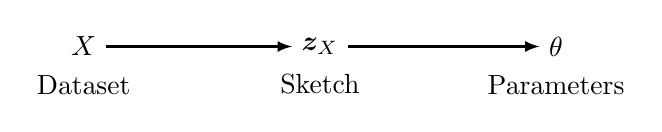
\begin{tikzpicture}
	% Place nodes
	\node [label=below:Dataset] (dataset) at (0,0) {$X$};
	\node [label=below:Sketch] (sketch) at (3,0) {$\Vec{z}_X$};
	\node [label=below:Parameters] (parameters) at (6,0) {$\theta$};
	
	% Draw edges
	\draw [->, thick, -latex] (dataset) -- (sketch);
	\draw [->, thick, -latex] (sketch) -- (parameters);
	\end{tikzpicture}
	\caption{The compressive learning workflow.}
	\label{fig:CL}
	\end {figure}

More precisely, CL comprises two steps (Figure \ref{fig:CL}):
\begin{enumerate}
	\item \textbf{Sketching:} The dataset $X = \{\Vec{x}_i \: | \: i = 1, ..., n\}$ (where we assume $\Vec{x}_i \in \bb R^d$) is compressed as a sketch vector that we note $\Vec{z}_X$, defined as the average over the dataset of some features $\Phi(\Vec{x}_i)$ (the function $\Phi : \mathbb R^d \mapsto \mathbb C^m$ or $\bb R^m$ computes $m$ features, possibly complex):
		\begin{equation}
		\label{eq:sketching}
		\Vec{z}_X := \frac{1}{n} \sum_{i = 1}^n \Phi(\Vec{x}_i).
		\end{equation}
	Since this is a simple averaging, sketching can be done on different chunks of $X$ independently, which is quite handy in distributed or streaming applications.
	\item \textbf{Learning:} The target model parameters $\theta$ are then obtained by some algorithm $\Delta$ that operates \emph{only} on this sketch,
		\begin{equation}
			\theta = \Delta(\Vec{z}_X).
		\end{equation}
		Typically, this involves solving some optimization problem $\min_{\theta} f(\theta ; \Vec{z}_X)$.
\end{enumerate}

\noindent In the following, these steps are explained intuitively, the formal details being introduced only when needed; for a more solid/exhaustive overview of compressive learning, see \cite{gribonval2017compressive}.

% TODO explain how it is structured, how to use


\subsection{Requirements}
The \pycle~package is built on standard Python scientific computing libraries: \code{numpy}, \code{scipy} and \code{matplotlib}; if you don't already have them installed, follow the instructions at \url{https://www.scipy.org/install.html}. %

% todo latest versions?

% You can install those packages by...

\subsection{Toolbox organization}
The \pycle toolbox is a collection of several submodules:
\begin{enumerate}
	\item The \code{sketching.py} module instantiates feature maps then computes the sketch of datasets with it.
	\item The \code{compressive\_learning.py} module contains the actual ``learning'' methods, extracting the desired parameters from the sketch.
	\item The \code{utils.py} module contains miscellaneous auxiliary functions, amongst others for generating synthetic datasets and evaluate the obtained solutions (as well quantitatively with well-defined metrics as qualitatively with visualization tools).
	\item Finally, the \code{third\_party.py} module serves to group code chunks used by \pycle that are written by other developers but not published as independent packages.
\end{enumerate}



\section{A tutorial tour of \pycle}
Let's explore the core submodules of \code{pycle}! Our focus here is understanding, so this section is a high-level tutorial rather than an exhaustive enumeration of what's inside the toolbox. %(however, section \ref{sec:documentation} is a methodical list of all the toolbox features). 

\subsection{Sketching dataset with the \code{sketching.py} submodule} 
To use the \code{sketching} submodule, you first need to import it (to spare me some typing, I personally like tu use \code{sk} as shorthand). Usual sketching as defined in~\eqref{eq:sketching} is simply done by calling \code{sk.computeSketch}. In practice it typically looks like this (we will fill in the dots later):
\begin{lstlisting}
import pycle.sketching as sk # import the sketching submodule

X = ...    # load a numpy array of dimension (n,d)
Phi = ... # sketch feature map, see later

z = sk.computeSketch(X,Phi) # z is a numpy array containing the sketch
\end{lstlisting}

\noindent As you might have guessed, \code{sk.computeSketch} requires two arguments: the dataset and the feature map. Let's start with the simplest one: the dataset $X$ should be given as a 2-d numpy array of dimensions $(n,d)$, i.e., number of examples times their dimension\footnote{\textbf{Matrix representation conventions:}
We follow the same convention as most mainstream Python machine learning modules: the dataset, mathematically described as $X = (\Vec{x}_i \in \mathbb R^d)_{i = 1}^n \in \mathbb R^{d \times n}$, is represented by a numpy array of shape $(n,d)$. In particular, \code{X[0]} references $\Vec{x_1}$: note the awkward inversion of dimension order. For matrices that don't represent datasets (e.g., $\Omega$ in the examples below), we stick to the mathematical convention instead, i.e., a matrix of the type $\mathbb R^{a \times b}$ is represented by a numpy array of shape $(a,b)$.}.

The feature map argument can be specified in one of the two following ways. Either---and this is the method I recommend---you give an instance of a \code{FeatureMap} object (explained below), or you directly provide a callable Python function (e.g., to compute the second-order moments for the sketch, write \code{Phi = lambda x: x**2}). Note that the second method is proposed for research purposes, in the case you want to construct a custom feature map that cannot be instantiated with the methods provided within the \code{FeatureMap} class\footnote{\textbf{FeatureMap objects:}
Why do we use \code{FeatureMap} objects instead of (Python) functions to represent... well, (mathematical) functions? Because we often require additional metadata/methods about $\Phi$ (e.g., target dimension $m$, jacobian $\nabla\Phi$,...). All these parameters and methods are conveniently packaged inside \code{FeatureMap} objects.}.

\emph{Voil�}, you know the basics of how the \code{sketching} submodule is used! Well, OK, all we saw was a function that computes an average, but hey, that's like, the essence of sketching, it's not my fault. Luckily for you, \code{sketching} has much more to offer. First and foremost, I'll demonstrate the whole zoo of feature maps that are readily available---I promise you, you'll construct your \code{FeatureMap} object $\Phi$ in no more than two lines of code. After this comes more advanced methods of the toolbox that you may not need right away: I'll show how to automatically select the \emph{scale hyper-parameter} in the aforementioned feature maps (which in practice can be hard to guess \emph{a priori}); I'll then finally explain \code{pycle}s functions for sketching with Differential Privacy guarantees. 

\subsubsection{Painless instantiation of standard feature maps: the \code{SimpleFeatureMap} class}
All feature maps used in CL up to now are of the following form, which we call ``Simple Feature Map'',
\begin{equation}
\Phi(\Vec{x}) = f(\Omega^T\Vec{x} + \Vec{\xi}), \quad \text{where} \quad \Omega = [\Vec{\omega}_1, \cdots, \Vec{\omega}_m] \in \mathbb{R}^{d \times m}, \: \Vec{\xi} = [\xi_1, \cdots, \xi_m]^T \in \mathbb{R}^{m},
\end{equation}
and $f$ is a point-wise nonlinearity (i.e., $\Phi_j(\Vec{x}) = f(\Vec{\omega}_j^T\Vec{x} + \xi_j)$ for all $j$). One way to interpret this map is to associate it with a one-layer neural network (where we don't necessarily learn the ``weights'' $\Omega$). You can instantiate such a nonlinearity in \code{pycle} in the following way:
\begin{lstlisting}
import pycle.sketching as sk

f = ...       # nonlinearity (Python function, tuple or string)
Omega = ...   # (d,m) numpy array
xi = ...      # (m,) numpy array
Phi = sk.SimpleFeatureMap(f, Omega, xi)
\end{lstlisting}

Moreover, the ``usual'' arguments for this simple feature map can be easily called, as we explain below.
\begin{itemize}
	\item \textbf{Nonlinearity:} you can simply pass in any Python function $\bb R \mapsto \bb C$ or $\bb R$. However, computing the gradient\footnote{Noting the Jacobian matrix $\nabla \Phi(\Vec{x}) = [\nabla \Phi_1(\Vec{x}) , \cdots , \nabla \Phi_m(\Vec{x}) ] \in \bb R^{d \times m}$ and $f'(t) = \frac{\mathrm{d}f(t)}{\mathrm{d}t}$ applied component-wise, we have $ \nabla \Phi(\Vec{x}) = \mathrm{diag} \left( f'(\Omega^T \Vec{x} + \Vec{\xi})\right) \cdot \Omega.$} $\nabla\Phi$ requires $\frac{\mathrm{d}f(t)}{\mathrm{d}t}$; you can also pass in a tuple of functions $(f,\frac{\mathrm{d}f(t)}{\mathrm{d}t})$ so that you can use gradient-based CL methods later. Lastly, you can use one of the predefined nonlinearities by passing a string matching one of the implemented nonlinearities. Those are : ...
	\item \textbf{Projection:} 
	\item dithering
\end{itemize}

\subsubsection{Designing the sampling pattern in the feature maps: the \code{estimateSigma} function}

\subsubsection{Guaranteeing the Differential Privacy of sketching: the \code{computeSketch\_DP} function}


% Explain the FeatureMap

% Come back to the code

% Privacy

\subsection{Learning from the sketch with the \code{compressive\_learning.py} submodule} 

\subsection{Utilities} 


%\section{Documentation}
%\label{sec:documentation}
%\subsection{Sketching methods} 

%\subsection{Learning tools} 

%\subsection{Utilities} 




\section{Conclusion: going further}
My primary goals for \code{pycle} are that it should be:
\begin{itemize}
	\item \textbf{intuitive to use:} practitioners with no background knowledge in compressive learning and little experience in Python should be able to use it to implement compressive learning in their own projects;
	\item \textbf{flexible to new features:} researchers with interest in compressive learning (that want to try out new methods/techniques in CL) should be able to easily extend this code to suit their own needs, without having to re-write things from scratch (and eventually, suggesting to add some features to the toolbox);
	\item \textbf{efficient to run:} the main motivation of compressive learning is based on the fact that it can be much more memory- and time-efficient than traditional learning methods, so the performances of the toolbox should fulfill that promise (note: this goal is still a challenge for me, this item is rather wishful thinking). 
\end{itemize}
With this in mind, if you have any suggestions to improve the toolbox, please don't hesitate to contact me!

\newpage
\bibliography{guidebib.bib}
\bibliographystyle{ieeetr}


\end{document}
